% Options for packages loaded elsewhere
\PassOptionsToPackage{unicode}{hyperref}
\PassOptionsToPackage{hyphens}{url}
%
\documentclass[
]{article}
\usepackage{lmodern}
\usepackage{amssymb,amsmath}
\usepackage{ifxetex,ifluatex}
\ifnum 0\ifxetex 1\fi\ifluatex 1\fi=0 % if pdftex
  \usepackage[T1]{fontenc}
  \usepackage[utf8]{inputenc}
  \usepackage{textcomp} % provide euro and other symbols
\else % if luatex or xetex
  \usepackage{unicode-math}
  \defaultfontfeatures{Scale=MatchLowercase}
  \defaultfontfeatures[\rmfamily]{Ligatures=TeX,Scale=1}
\fi
% Use upquote if available, for straight quotes in verbatim environments
\IfFileExists{upquote.sty}{\usepackage{upquote}}{}
\IfFileExists{microtype.sty}{% use microtype if available
  \usepackage[]{microtype}
  \UseMicrotypeSet[protrusion]{basicmath} % disable protrusion for tt fonts
}{}
\makeatletter
\@ifundefined{KOMAClassName}{% if non-KOMA class
  \IfFileExists{parskip.sty}{%
    \usepackage{parskip}
  }{% else
    \setlength{\parindent}{0pt}
    \setlength{\parskip}{6pt plus 2pt minus 1pt}}
}{% if KOMA class
  \KOMAoptions{parskip=half}}
\makeatother
\usepackage{xcolor}
\IfFileExists{xurl.sty}{\usepackage{xurl}}{} % add URL line breaks if available
\IfFileExists{bookmark.sty}{\usepackage{bookmark}}{\usepackage{hyperref}}
\hypersetup{
  pdftitle={Visualization 1: Descriptive Statistics},
  pdfauthor={Fan Lu \& Gento Kato},
  hidelinks,
  pdfcreator={LaTeX via pandoc}}
\urlstyle{same} % disable monospaced font for URLs
\usepackage[margin=1in]{geometry}
\usepackage{color}
\usepackage{fancyvrb}
\newcommand{\VerbBar}{|}
\newcommand{\VERB}{\Verb[commandchars=\\\{\}]}
\DefineVerbatimEnvironment{Highlighting}{Verbatim}{commandchars=\\\{\}}
% Add ',fontsize=\small' for more characters per line
\usepackage{framed}
\definecolor{shadecolor}{RGB}{248,248,248}
\newenvironment{Shaded}{\begin{snugshade}}{\end{snugshade}}
\newcommand{\AlertTok}[1]{\textcolor[rgb]{0.94,0.16,0.16}{#1}}
\newcommand{\AnnotationTok}[1]{\textcolor[rgb]{0.56,0.35,0.01}{\textbf{\textit{#1}}}}
\newcommand{\AttributeTok}[1]{\textcolor[rgb]{0.77,0.63,0.00}{#1}}
\newcommand{\BaseNTok}[1]{\textcolor[rgb]{0.00,0.00,0.81}{#1}}
\newcommand{\BuiltInTok}[1]{#1}
\newcommand{\CharTok}[1]{\textcolor[rgb]{0.31,0.60,0.02}{#1}}
\newcommand{\CommentTok}[1]{\textcolor[rgb]{0.56,0.35,0.01}{\textit{#1}}}
\newcommand{\CommentVarTok}[1]{\textcolor[rgb]{0.56,0.35,0.01}{\textbf{\textit{#1}}}}
\newcommand{\ConstantTok}[1]{\textcolor[rgb]{0.00,0.00,0.00}{#1}}
\newcommand{\ControlFlowTok}[1]{\textcolor[rgb]{0.13,0.29,0.53}{\textbf{#1}}}
\newcommand{\DataTypeTok}[1]{\textcolor[rgb]{0.13,0.29,0.53}{#1}}
\newcommand{\DecValTok}[1]{\textcolor[rgb]{0.00,0.00,0.81}{#1}}
\newcommand{\DocumentationTok}[1]{\textcolor[rgb]{0.56,0.35,0.01}{\textbf{\textit{#1}}}}
\newcommand{\ErrorTok}[1]{\textcolor[rgb]{0.64,0.00,0.00}{\textbf{#1}}}
\newcommand{\ExtensionTok}[1]{#1}
\newcommand{\FloatTok}[1]{\textcolor[rgb]{0.00,0.00,0.81}{#1}}
\newcommand{\FunctionTok}[1]{\textcolor[rgb]{0.00,0.00,0.00}{#1}}
\newcommand{\ImportTok}[1]{#1}
\newcommand{\InformationTok}[1]{\textcolor[rgb]{0.56,0.35,0.01}{\textbf{\textit{#1}}}}
\newcommand{\KeywordTok}[1]{\textcolor[rgb]{0.13,0.29,0.53}{\textbf{#1}}}
\newcommand{\NormalTok}[1]{#1}
\newcommand{\OperatorTok}[1]{\textcolor[rgb]{0.81,0.36,0.00}{\textbf{#1}}}
\newcommand{\OtherTok}[1]{\textcolor[rgb]{0.56,0.35,0.01}{#1}}
\newcommand{\PreprocessorTok}[1]{\textcolor[rgb]{0.56,0.35,0.01}{\textit{#1}}}
\newcommand{\RegionMarkerTok}[1]{#1}
\newcommand{\SpecialCharTok}[1]{\textcolor[rgb]{0.00,0.00,0.00}{#1}}
\newcommand{\SpecialStringTok}[1]{\textcolor[rgb]{0.31,0.60,0.02}{#1}}
\newcommand{\StringTok}[1]{\textcolor[rgb]{0.31,0.60,0.02}{#1}}
\newcommand{\VariableTok}[1]{\textcolor[rgb]{0.00,0.00,0.00}{#1}}
\newcommand{\VerbatimStringTok}[1]{\textcolor[rgb]{0.31,0.60,0.02}{#1}}
\newcommand{\WarningTok}[1]{\textcolor[rgb]{0.56,0.35,0.01}{\textbf{\textit{#1}}}}
\usepackage{graphicx,grffile}
\makeatletter
\def\maxwidth{\ifdim\Gin@nat@width>\linewidth\linewidth\else\Gin@nat@width\fi}
\def\maxheight{\ifdim\Gin@nat@height>\textheight\textheight\else\Gin@nat@height\fi}
\makeatother
% Scale images if necessary, so that they will not overflow the page
% margins by default, and it is still possible to overwrite the defaults
% using explicit options in \includegraphics[width, height, ...]{}
\setkeys{Gin}{width=\maxwidth,height=\maxheight,keepaspectratio}
% Set default figure placement to htbp
\makeatletter
\def\fps@figure{htbp}
\makeatother
\setlength{\emergencystretch}{3em} % prevent overfull lines
\providecommand{\tightlist}{%
  \setlength{\itemsep}{0pt}\setlength{\parskip}{0pt}}
\setcounter{secnumdepth}{-\maxdimen} % remove section numbering
\usepackage{bookmark}
\usepackage{xltxtra}
\usepackage{zxjatype}
\usepackage[ipa]{zxjafont}

\title{Visualization 1: Descriptive Statistics}
\author{Fan Lu \& Gento Kato}
\date{January 26, 2020}

\begin{document}
\maketitle

\hypertarget{preparation}{%
\section{Preparation}\label{preparation}}

\begin{Shaded}
\begin{Highlighting}[]
\CommentTok{## Clean Up Space}
\KeywordTok{rm}\NormalTok{(}\DataTypeTok{list=}\KeywordTok{ls}\NormalTok{())}

\CommentTok{## Set Working Directory (Automatically) ##}
\KeywordTok{require}\NormalTok{(rstudioapi); }\KeywordTok{require}\NormalTok{(rprojroot)}
\ControlFlowTok{if}\NormalTok{ (rstudioapi}\OperatorTok{::}\KeywordTok{isAvailable}\NormalTok{()}\OperatorTok{==}\OtherTok{TRUE}\NormalTok{) \{}
  \KeywordTok{setwd}\NormalTok{(}\KeywordTok{dirname}\NormalTok{(rstudioapi}\OperatorTok{::}\KeywordTok{getActiveDocumentContext}\NormalTok{()}\OperatorTok{$}\NormalTok{path)); }
\NormalTok{\} }
\NormalTok{projdir <-}\StringTok{ }\KeywordTok{find_root}\NormalTok{(}\KeywordTok{has_file}\NormalTok{(}\StringTok{"thisishome.txt"}\NormalTok{))}
\KeywordTok{cat}\NormalTok{(}\KeywordTok{paste}\NormalTok{(}\StringTok{"Working Directory Set to:}\CharTok{\textbackslash{}n}\StringTok{"}\NormalTok{,projdir))}
\end{Highlighting}
\end{Shaded}

\begin{verbatim}
## Working Directory Set to:
##  /home/gentok/GoogleDrive/Projects/Fan-Gento-Lab/ForeignerJapan
\end{verbatim}

\begin{Shaded}
\begin{Highlighting}[]
\KeywordTok{setwd}\NormalTok{(projdir)}

\CommentTok{## Original Data}
\NormalTok{datadir1a <-}\StringTok{ }\KeywordTok{paste0}\NormalTok{(projdir, }\StringTok{"/data/sifcct_zip_latest_v5.rds"}\NormalTok{)}
\NormalTok{datadir1b <-}\StringTok{ }\KeywordTok{paste0}\NormalTok{(projdir, }\StringTok{"/data/sifcct_zip_latest_panel_v5.rds"}\NormalTok{)}
\NormalTok{datadir2 <-}\StringTok{ }\KeywordTok{paste0}\NormalTok{(projdir, }\StringTok{"/data/mail_zip_latest_v5.rds"}\NormalTok{)}

\CommentTok{## packages}
\KeywordTok{library}\NormalTok{(ggplot2)}
\end{Highlighting}
\end{Shaded}

\hypertarget{import-and-clean-data}{%
\section{Import and clean data}\label{import-and-clean-data}}

\begin{Shaded}
\begin{Highlighting}[]
\CommentTok{###################}
\CommentTok{## SIFCCT Online ##}
\CommentTok{###################}

\NormalTok{sifcct <-}\StringTok{ }\KeywordTok{rbind}\NormalTok{(}\KeywordTok{readRDS}\NormalTok{(datadir1a),}\KeywordTok{readRDS}\NormalTok{(datadir1b))}

\CommentTok{## Knowledge Variable (Replaced)}
\NormalTok{sifcct}\OperatorTok{$}\NormalTok{knowledge[sifcct}\OperatorTok{$}\NormalTok{panel}\OperatorTok{==}\DecValTok{1} \OperatorTok{&}\StringTok{ }\NormalTok{sifcct}\OperatorTok{$}\NormalTok{wave}\OperatorTok{==}\DecValTok{2}\NormalTok{] <-}\StringTok{ }\NormalTok{sifcct}\OperatorTok{$}\NormalTok{knowledge[sifcct}\OperatorTok{$}\NormalTok{panel}\OperatorTok{==}\DecValTok{1} \OperatorTok{&}\StringTok{ }\NormalTok{sifcct}\OperatorTok{$}\NormalTok{wave}\OperatorTok{==}\DecValTok{1}\NormalTok{][}\KeywordTok{match}\NormalTok{(sifcct}\OperatorTok{$}\NormalTok{panelid[sifcct}\OperatorTok{$}\NormalTok{panel}\OperatorTok{==}\DecValTok{1} \OperatorTok{&}\StringTok{ }\NormalTok{sifcct}\OperatorTok{$}\NormalTok{wave}\OperatorTok{==}\DecValTok{2}\NormalTok{],sifcct}\OperatorTok{$}\NormalTok{panelid[sifcct}\OperatorTok{$}\NormalTok{panel}\OperatorTok{==}\DecValTok{1} \OperatorTok{&}\StringTok{ }\NormalTok{sifcct}\OperatorTok{$}\NormalTok{wave}\OperatorTok{==}\DecValTok{1}\NormalTok{])]}
\NormalTok{sifcct}\OperatorTok{$}\NormalTok{knowledge[sifcct}\OperatorTok{$}\NormalTok{panel}\OperatorTok{==}\DecValTok{1} \OperatorTok{&}\StringTok{ }\NormalTok{sifcct}\OperatorTok{$}\NormalTok{wave}\OperatorTok{==}\DecValTok{3}\NormalTok{] <-}\StringTok{ }\NormalTok{sifcct}\OperatorTok{$}\NormalTok{knowledge[sifcct}\OperatorTok{$}\NormalTok{panel}\OperatorTok{==}\DecValTok{1} \OperatorTok{&}\StringTok{ }\NormalTok{sifcct}\OperatorTok{$}\NormalTok{wave}\OperatorTok{==}\DecValTok{1}\NormalTok{][}\KeywordTok{match}\NormalTok{(sifcct}\OperatorTok{$}\NormalTok{panelid[sifcct}\OperatorTok{$}\NormalTok{panel}\OperatorTok{==}\DecValTok{1} \OperatorTok{&}\StringTok{ }\NormalTok{sifcct}\OperatorTok{$}\NormalTok{wave}\OperatorTok{==}\DecValTok{3}\NormalTok{],sifcct}\OperatorTok{$}\NormalTok{panelid[sifcct}\OperatorTok{$}\NormalTok{panel}\OperatorTok{==}\DecValTok{1} \OperatorTok{&}\StringTok{ }\NormalTok{sifcct}\OperatorTok{$}\NormalTok{wave}\OperatorTok{==}\DecValTok{1}\NormalTok{])]}
\NormalTok{sifcct}\OperatorTok{$}\NormalTok{knowledge[sifcct}\OperatorTok{$}\NormalTok{panel}\OperatorTok{==}\DecValTok{1} \OperatorTok{&}\StringTok{ }\NormalTok{sifcct}\OperatorTok{$}\NormalTok{wave}\OperatorTok{==}\DecValTok{4}\NormalTok{] <-}\StringTok{ }\NormalTok{sifcct}\OperatorTok{$}\NormalTok{knowledge[sifcct}\OperatorTok{$}\NormalTok{panel}\OperatorTok{==}\DecValTok{1} \OperatorTok{&}\StringTok{ }\NormalTok{sifcct}\OperatorTok{$}\NormalTok{wave}\OperatorTok{==}\DecValTok{1}\NormalTok{][}\KeywordTok{match}\NormalTok{(sifcct}\OperatorTok{$}\NormalTok{panelid[sifcct}\OperatorTok{$}\NormalTok{panel}\OperatorTok{==}\DecValTok{1} \OperatorTok{&}\StringTok{ }\NormalTok{sifcct}\OperatorTok{$}\NormalTok{wave}\OperatorTok{==}\DecValTok{4}\NormalTok{],sifcct}\OperatorTok{$}\NormalTok{panelid[sifcct}\OperatorTok{$}\NormalTok{panel}\OperatorTok{==}\DecValTok{1} \OperatorTok{&}\StringTok{ }\NormalTok{sifcct}\OperatorTok{$}\NormalTok{wave}\OperatorTok{==}\DecValTok{1}\NormalTok{])]}
\NormalTok{sifcct}\OperatorTok{$}\NormalTok{knowledge[sifcct}\OperatorTok{$}\NormalTok{panel}\OperatorTok{==}\DecValTok{1} \OperatorTok{&}\StringTok{ }\NormalTok{sifcct}\OperatorTok{$}\NormalTok{wave}\OperatorTok{==}\DecValTok{5}\NormalTok{] <-}\StringTok{ }\NormalTok{sifcct}\OperatorTok{$}\NormalTok{knowledge[sifcct}\OperatorTok{$}\NormalTok{panel}\OperatorTok{==}\DecValTok{1} \OperatorTok{&}\StringTok{ }\NormalTok{sifcct}\OperatorTok{$}\NormalTok{wave}\OperatorTok{==}\DecValTok{1}\NormalTok{][}\KeywordTok{match}\NormalTok{(sifcct}\OperatorTok{$}\NormalTok{panelid[sifcct}\OperatorTok{$}\NormalTok{panel}\OperatorTok{==}\DecValTok{1} \OperatorTok{&}\StringTok{ }\NormalTok{sifcct}\OperatorTok{$}\NormalTok{wave}\OperatorTok{==}\DecValTok{5}\NormalTok{],sifcct}\OperatorTok{$}\NormalTok{panelid[sifcct}\OperatorTok{$}\NormalTok{panel}\OperatorTok{==}\DecValTok{1} \OperatorTok{&}\StringTok{ }\NormalTok{sifcct}\OperatorTok{$}\NormalTok{wave}\OperatorTok{==}\DecValTok{1}\NormalTok{])]}
\NormalTok{sifcct}\OperatorTok{$}\NormalTok{knowledge[sifcct}\OperatorTok{$}\NormalTok{panel}\OperatorTok{==}\DecValTok{1} \OperatorTok{&}\StringTok{ }\NormalTok{sifcct}\OperatorTok{$}\NormalTok{wave}\OperatorTok{==}\DecValTok{6}\NormalTok{] <-}\StringTok{ }\NormalTok{sifcct}\OperatorTok{$}\NormalTok{knowledge[sifcct}\OperatorTok{$}\NormalTok{panel}\OperatorTok{==}\DecValTok{1} \OperatorTok{&}\StringTok{ }\NormalTok{sifcct}\OperatorTok{$}\NormalTok{wave}\OperatorTok{==}\DecValTok{1}\NormalTok{][}\KeywordTok{match}\NormalTok{(sifcct}\OperatorTok{$}\NormalTok{panelid[sifcct}\OperatorTok{$}\NormalTok{panel}\OperatorTok{==}\DecValTok{1} \OperatorTok{&}\StringTok{ }\NormalTok{sifcct}\OperatorTok{$}\NormalTok{wave}\OperatorTok{==}\DecValTok{6}\NormalTok{],sifcct}\OperatorTok{$}\NormalTok{panelid[sifcct}\OperatorTok{$}\NormalTok{panel}\OperatorTok{==}\DecValTok{1} \OperatorTok{&}\StringTok{ }\NormalTok{sifcct}\OperatorTok{$}\NormalTok{wave}\OperatorTok{==}\DecValTok{1}\NormalTok{])]}
\NormalTok{sifcct}\OperatorTok{$}\NormalTok{knowledge[sifcct}\OperatorTok{$}\NormalTok{panel}\OperatorTok{==}\DecValTok{1} \OperatorTok{&}\StringTok{ }\NormalTok{sifcct}\OperatorTok{$}\NormalTok{wave}\OperatorTok{==}\DecValTok{7}\NormalTok{] <-}\StringTok{ }\NormalTok{sifcct}\OperatorTok{$}\NormalTok{knowledge[sifcct}\OperatorTok{$}\NormalTok{panel}\OperatorTok{==}\DecValTok{1} \OperatorTok{&}\StringTok{ }\NormalTok{sifcct}\OperatorTok{$}\NormalTok{wave}\OperatorTok{==}\DecValTok{1}\NormalTok{][}\KeywordTok{match}\NormalTok{(sifcct}\OperatorTok{$}\NormalTok{panelid[sifcct}\OperatorTok{$}\NormalTok{panel}\OperatorTok{==}\DecValTok{1} \OperatorTok{&}\StringTok{ }\NormalTok{sifcct}\OperatorTok{$}\NormalTok{wave}\OperatorTok{==}\DecValTok{7}\NormalTok{],sifcct}\OperatorTok{$}\NormalTok{panelid[sifcct}\OperatorTok{$}\NormalTok{panel}\OperatorTok{==}\DecValTok{1} \OperatorTok{&}\StringTok{ }\NormalTok{sifcct}\OperatorTok{$}\NormalTok{wave}\OperatorTok{==}\DecValTok{1}\NormalTok{])]}
\NormalTok{sifcct}\OperatorTok{$}\NormalTok{knowledge[sifcct}\OperatorTok{$}\NormalTok{panel}\OperatorTok{==}\DecValTok{1} \OperatorTok{&}\StringTok{ }\NormalTok{sifcct}\OperatorTok{$}\NormalTok{wave}\OperatorTok{==}\DecValTok{8}\NormalTok{] <-}\StringTok{ }\NormalTok{sifcct}\OperatorTok{$}\NormalTok{knowledge[sifcct}\OperatorTok{$}\NormalTok{panel}\OperatorTok{==}\DecValTok{1} \OperatorTok{&}\StringTok{ }\NormalTok{sifcct}\OperatorTok{$}\NormalTok{wave}\OperatorTok{==}\DecValTok{1}\NormalTok{][}\KeywordTok{match}\NormalTok{(sifcct}\OperatorTok{$}\NormalTok{panelid[sifcct}\OperatorTok{$}\NormalTok{panel}\OperatorTok{==}\DecValTok{1} \OperatorTok{&}\StringTok{ }\NormalTok{sifcct}\OperatorTok{$}\NormalTok{wave}\OperatorTok{==}\DecValTok{8}\NormalTok{],sifcct}\OperatorTok{$}\NormalTok{panelid[sifcct}\OperatorTok{$}\NormalTok{panel}\OperatorTok{==}\DecValTok{1} \OperatorTok{&}\StringTok{ }\NormalTok{sifcct}\OperatorTok{$}\NormalTok{wave}\OperatorTok{==}\DecValTok{1}\NormalTok{])]}
\NormalTok{sifcct}\OperatorTok{$}\NormalTok{knowledge[sifcct}\OperatorTok{$}\NormalTok{panel}\OperatorTok{==}\DecValTok{1} \OperatorTok{&}\StringTok{ }\NormalTok{sifcct}\OperatorTok{$}\NormalTok{wave}\OperatorTok{==}\DecValTok{9}\NormalTok{] <-}\StringTok{ }\NormalTok{sifcct}\OperatorTok{$}\NormalTok{knowledge[sifcct}\OperatorTok{$}\NormalTok{panel}\OperatorTok{==}\DecValTok{1} \OperatorTok{&}\StringTok{ }\NormalTok{sifcct}\OperatorTok{$}\NormalTok{wave}\OperatorTok{==}\DecValTok{1}\NormalTok{][}\KeywordTok{match}\NormalTok{(sifcct}\OperatorTok{$}\NormalTok{panelid[sifcct}\OperatorTok{$}\NormalTok{panel}\OperatorTok{==}\DecValTok{1} \OperatorTok{&}\StringTok{ }\NormalTok{sifcct}\OperatorTok{$}\NormalTok{wave}\OperatorTok{==}\DecValTok{9}\NormalTok{],sifcct}\OperatorTok{$}\NormalTok{panelid[sifcct}\OperatorTok{$}\NormalTok{panel}\OperatorTok{==}\DecValTok{1} \OperatorTok{&}\StringTok{ }\NormalTok{sifcct}\OperatorTok{$}\NormalTok{wave}\OperatorTok{==}\DecValTok{1}\NormalTok{])]}
\NormalTok{sifcct}\OperatorTok{$}\NormalTok{knowledge[sifcct}\OperatorTok{$}\NormalTok{panel}\OperatorTok{==}\DecValTok{1} \OperatorTok{&}\StringTok{ }\NormalTok{sifcct}\OperatorTok{$}\NormalTok{wave}\OperatorTok{==}\DecValTok{10}\NormalTok{] <-}\StringTok{ }\NormalTok{sifcct}\OperatorTok{$}\NormalTok{knowledge[sifcct}\OperatorTok{$}\NormalTok{panel}\OperatorTok{==}\DecValTok{1} \OperatorTok{&}\StringTok{ }\NormalTok{sifcct}\OperatorTok{$}\NormalTok{wave}\OperatorTok{==}\DecValTok{1}\NormalTok{][}\KeywordTok{match}\NormalTok{(sifcct}\OperatorTok{$}\NormalTok{panelid[sifcct}\OperatorTok{$}\NormalTok{panel}\OperatorTok{==}\DecValTok{1} \OperatorTok{&}\StringTok{ }\NormalTok{sifcct}\OperatorTok{$}\NormalTok{wave}\OperatorTok{==}\DecValTok{10}\NormalTok{],sifcct}\OperatorTok{$}\NormalTok{panelid[sifcct}\OperatorTok{$}\NormalTok{panel}\OperatorTok{==}\DecValTok{1} \OperatorTok{&}\StringTok{ }\NormalTok{sifcct}\OperatorTok{$}\NormalTok{wave}\OperatorTok{==}\DecValTok{1}\NormalTok{])]}
\NormalTok{sifcct}\OperatorTok{$}\NormalTok{knowledge[sifcct}\OperatorTok{$}\NormalTok{panel}\OperatorTok{==}\DecValTok{1} \OperatorTok{&}\StringTok{ }\NormalTok{sifcct}\OperatorTok{$}\NormalTok{wave}\OperatorTok{==}\DecValTok{11}\NormalTok{] <-}\StringTok{ }\NormalTok{sifcct}\OperatorTok{$}\NormalTok{knowledge[sifcct}\OperatorTok{$}\NormalTok{panel}\OperatorTok{==}\DecValTok{1} \OperatorTok{&}\StringTok{ }\NormalTok{sifcct}\OperatorTok{$}\NormalTok{wave}\OperatorTok{==}\DecValTok{1}\NormalTok{][}\KeywordTok{match}\NormalTok{(sifcct}\OperatorTok{$}\NormalTok{panelid[sifcct}\OperatorTok{$}\NormalTok{panel}\OperatorTok{==}\DecValTok{1} \OperatorTok{&}\StringTok{ }\NormalTok{sifcct}\OperatorTok{$}\NormalTok{wave}\OperatorTok{==}\DecValTok{11}\NormalTok{],sifcct}\OperatorTok{$}\NormalTok{panelid[sifcct}\OperatorTok{$}\NormalTok{panel}\OperatorTok{==}\DecValTok{1} \OperatorTok{&}\StringTok{ }\NormalTok{sifcct}\OperatorTok{$}\NormalTok{wave}\OperatorTok{==}\DecValTok{1}\NormalTok{])]}
\NormalTok{sifcct}\OperatorTok{$}\NormalTok{knowledge[sifcct}\OperatorTok{$}\NormalTok{panel}\OperatorTok{==}\DecValTok{1} \OperatorTok{&}\StringTok{ }\NormalTok{sifcct}\OperatorTok{$}\NormalTok{wave}\OperatorTok{==}\DecValTok{12}\NormalTok{] <-}\StringTok{ }\NormalTok{sifcct}\OperatorTok{$}\NormalTok{knowledge[sifcct}\OperatorTok{$}\NormalTok{panel}\OperatorTok{==}\DecValTok{1} \OperatorTok{&}\StringTok{ }\NormalTok{sifcct}\OperatorTok{$}\NormalTok{wave}\OperatorTok{==}\DecValTok{1}\NormalTok{][}\KeywordTok{match}\NormalTok{(sifcct}\OperatorTok{$}\NormalTok{panelid[sifcct}\OperatorTok{$}\NormalTok{panel}\OperatorTok{==}\DecValTok{1} \OperatorTok{&}\StringTok{ }\NormalTok{sifcct}\OperatorTok{$}\NormalTok{wave}\OperatorTok{==}\DecValTok{12}\NormalTok{],sifcct}\OperatorTok{$}\NormalTok{panelid[sifcct}\OperatorTok{$}\NormalTok{panel}\OperatorTok{==}\DecValTok{1} \OperatorTok{&}\StringTok{ }\NormalTok{sifcct}\OperatorTok{$}\NormalTok{wave}\OperatorTok{==}\DecValTok{1}\NormalTok{])]}
\CommentTok{## Knowledge Variable (Replaced)}
\NormalTok{sifcct}\OperatorTok{$}\NormalTok{knowledge[sifcct}\OperatorTok{$}\NormalTok{panel}\OperatorTok{==}\DecValTok{1} \OperatorTok{&}\StringTok{ }\NormalTok{sifcct}\OperatorTok{$}\NormalTok{wave}\OperatorTok{==}\DecValTok{14}\NormalTok{] <-}\StringTok{ }\NormalTok{sifcct}\OperatorTok{$}\NormalTok{knowledge[sifcct}\OperatorTok{$}\NormalTok{panel}\OperatorTok{==}\DecValTok{1} \OperatorTok{&}\StringTok{ }\NormalTok{sifcct}\OperatorTok{$}\NormalTok{wave}\OperatorTok{==}\DecValTok{13}\NormalTok{][}\KeywordTok{match}\NormalTok{(sifcct}\OperatorTok{$}\NormalTok{panelid[sifcct}\OperatorTok{$}\NormalTok{panel}\OperatorTok{==}\DecValTok{1} \OperatorTok{&}\StringTok{ }\NormalTok{sifcct}\OperatorTok{$}\NormalTok{wave}\OperatorTok{==}\DecValTok{14}\NormalTok{],sifcct}\OperatorTok{$}\NormalTok{panelid[sifcct}\OperatorTok{$}\NormalTok{panel}\OperatorTok{==}\DecValTok{1} \OperatorTok{&}\StringTok{ }\NormalTok{sifcct}\OperatorTok{$}\NormalTok{wave}\OperatorTok{==}\DecValTok{13}\NormalTok{])]}
\NormalTok{sifcct}\OperatorTok{$}\NormalTok{knowledge[sifcct}\OperatorTok{$}\NormalTok{panel}\OperatorTok{==}\DecValTok{1} \OperatorTok{&}\StringTok{ }\NormalTok{sifcct}\OperatorTok{$}\NormalTok{wave}\OperatorTok{==}\DecValTok{15}\NormalTok{] <-}\StringTok{ }\NormalTok{sifcct}\OperatorTok{$}\NormalTok{knowledge[sifcct}\OperatorTok{$}\NormalTok{panel}\OperatorTok{==}\DecValTok{1} \OperatorTok{&}\StringTok{ }\NormalTok{sifcct}\OperatorTok{$}\NormalTok{wave}\OperatorTok{==}\DecValTok{13}\NormalTok{][}\KeywordTok{match}\NormalTok{(sifcct}\OperatorTok{$}\NormalTok{panelid[sifcct}\OperatorTok{$}\NormalTok{panel}\OperatorTok{==}\DecValTok{1} \OperatorTok{&}\StringTok{ }\NormalTok{sifcct}\OperatorTok{$}\NormalTok{wave}\OperatorTok{==}\DecValTok{15}\NormalTok{],sifcct}\OperatorTok{$}\NormalTok{panelid[sifcct}\OperatorTok{$}\NormalTok{panel}\OperatorTok{==}\DecValTok{1} \OperatorTok{&}\StringTok{ }\NormalTok{sifcct}\OperatorTok{$}\NormalTok{wave}\OperatorTok{==}\DecValTok{13}\NormalTok{])]}
\NormalTok{sifcct}\OperatorTok{$}\NormalTok{knowledge[sifcct}\OperatorTok{$}\NormalTok{panel}\OperatorTok{==}\DecValTok{1} \OperatorTok{&}\StringTok{ }\NormalTok{sifcct}\OperatorTok{$}\NormalTok{wave}\OperatorTok{==}\DecValTok{16}\NormalTok{] <-}\StringTok{ }\NormalTok{sifcct}\OperatorTok{$}\NormalTok{knowledge[sifcct}\OperatorTok{$}\NormalTok{panel}\OperatorTok{==}\DecValTok{1} \OperatorTok{&}\StringTok{ }\NormalTok{sifcct}\OperatorTok{$}\NormalTok{wave}\OperatorTok{==}\DecValTok{13}\NormalTok{][}\KeywordTok{match}\NormalTok{(sifcct}\OperatorTok{$}\NormalTok{panelid[sifcct}\OperatorTok{$}\NormalTok{panel}\OperatorTok{==}\DecValTok{1} \OperatorTok{&}\StringTok{ }\NormalTok{sifcct}\OperatorTok{$}\NormalTok{wave}\OperatorTok{==}\DecValTok{16}\NormalTok{],sifcct}\OperatorTok{$}\NormalTok{panelid[sifcct}\OperatorTok{$}\NormalTok{panel}\OperatorTok{==}\DecValTok{1} \OperatorTok{&}\StringTok{ }\NormalTok{sifcct}\OperatorTok{$}\NormalTok{wave}\OperatorTok{==}\DecValTok{13}\NormalTok{])]}
\NormalTok{sifcct}\OperatorTok{$}\NormalTok{knowledge[sifcct}\OperatorTok{$}\NormalTok{panel}\OperatorTok{==}\DecValTok{1} \OperatorTok{&}\StringTok{ }\NormalTok{sifcct}\OperatorTok{$}\NormalTok{wave}\OperatorTok{==}\DecValTok{17}\NormalTok{] <-}\StringTok{ }\NormalTok{sifcct}\OperatorTok{$}\NormalTok{knowledge[sifcct}\OperatorTok{$}\NormalTok{panel}\OperatorTok{==}\DecValTok{1} \OperatorTok{&}\StringTok{ }\NormalTok{sifcct}\OperatorTok{$}\NormalTok{wave}\OperatorTok{==}\DecValTok{13}\NormalTok{][}\KeywordTok{match}\NormalTok{(sifcct}\OperatorTok{$}\NormalTok{panelid[sifcct}\OperatorTok{$}\NormalTok{panel}\OperatorTok{==}\DecValTok{1} \OperatorTok{&}\StringTok{ }\NormalTok{sifcct}\OperatorTok{$}\NormalTok{wave}\OperatorTok{==}\DecValTok{17}\NormalTok{],sifcct}\OperatorTok{$}\NormalTok{panelid[sifcct}\OperatorTok{$}\NormalTok{panel}\OperatorTok{==}\DecValTok{1} \OperatorTok{&}\StringTok{ }\NormalTok{sifcct}\OperatorTok{$}\NormalTok{wave}\OperatorTok{==}\DecValTok{13}\NormalTok{])]}
\NormalTok{sifcct}\OperatorTok{$}\NormalTok{knowledge[sifcct}\OperatorTok{$}\NormalTok{panel}\OperatorTok{==}\DecValTok{1} \OperatorTok{&}\StringTok{ }\NormalTok{sifcct}\OperatorTok{$}\NormalTok{wave}\OperatorTok{==}\DecValTok{18}\NormalTok{] <-}\StringTok{ }\NormalTok{sifcct}\OperatorTok{$}\NormalTok{knowledge[sifcct}\OperatorTok{$}\NormalTok{panel}\OperatorTok{==}\DecValTok{1} \OperatorTok{&}\StringTok{ }\NormalTok{sifcct}\OperatorTok{$}\NormalTok{wave}\OperatorTok{==}\DecValTok{13}\NormalTok{][}\KeywordTok{match}\NormalTok{(sifcct}\OperatorTok{$}\NormalTok{panelid[sifcct}\OperatorTok{$}\NormalTok{panel}\OperatorTok{==}\DecValTok{1} \OperatorTok{&}\StringTok{ }\NormalTok{sifcct}\OperatorTok{$}\NormalTok{wave}\OperatorTok{==}\DecValTok{18}\NormalTok{],sifcct}\OperatorTok{$}\NormalTok{panelid[sifcct}\OperatorTok{$}\NormalTok{panel}\OperatorTok{==}\DecValTok{1} \OperatorTok{&}\StringTok{ }\NormalTok{sifcct}\OperatorTok{$}\NormalTok{wave}\OperatorTok{==}\DecValTok{13}\NormalTok{])]}
\NormalTok{sifcct}\OperatorTok{$}\NormalTok{knowledge[sifcct}\OperatorTok{$}\NormalTok{panel}\OperatorTok{==}\DecValTok{1} \OperatorTok{&}\StringTok{ }\NormalTok{sifcct}\OperatorTok{$}\NormalTok{wave}\OperatorTok{==}\DecValTok{19}\NormalTok{] <-}\StringTok{ }\NormalTok{sifcct}\OperatorTok{$}\NormalTok{knowledge[sifcct}\OperatorTok{$}\NormalTok{panel}\OperatorTok{==}\DecValTok{1} \OperatorTok{&}\StringTok{ }\NormalTok{sifcct}\OperatorTok{$}\NormalTok{wave}\OperatorTok{==}\DecValTok{13}\NormalTok{][}\KeywordTok{match}\NormalTok{(sifcct}\OperatorTok{$}\NormalTok{panelid[sifcct}\OperatorTok{$}\NormalTok{panel}\OperatorTok{==}\DecValTok{1} \OperatorTok{&}\StringTok{ }\NormalTok{sifcct}\OperatorTok{$}\NormalTok{wave}\OperatorTok{==}\DecValTok{19}\NormalTok{],sifcct}\OperatorTok{$}\NormalTok{panelid[sifcct}\OperatorTok{$}\NormalTok{panel}\OperatorTok{==}\DecValTok{1} \OperatorTok{&}\StringTok{ }\NormalTok{sifcct}\OperatorTok{$}\NormalTok{wave}\OperatorTok{==}\DecValTok{13}\NormalTok{])]}
\NormalTok{sifcct}\OperatorTok{$}\NormalTok{knowledge[sifcct}\OperatorTok{$}\NormalTok{panel}\OperatorTok{==}\DecValTok{1} \OperatorTok{&}\StringTok{ }\NormalTok{sifcct}\OperatorTok{$}\NormalTok{wave}\OperatorTok{==}\DecValTok{20}\NormalTok{] <-}\StringTok{ }\NormalTok{sifcct}\OperatorTok{$}\NormalTok{knowledge[sifcct}\OperatorTok{$}\NormalTok{panel}\OperatorTok{==}\DecValTok{1} \OperatorTok{&}\StringTok{ }\NormalTok{sifcct}\OperatorTok{$}\NormalTok{wave}\OperatorTok{==}\DecValTok{13}\NormalTok{][}\KeywordTok{match}\NormalTok{(sifcct}\OperatorTok{$}\NormalTok{panelid[sifcct}\OperatorTok{$}\NormalTok{panel}\OperatorTok{==}\DecValTok{1} \OperatorTok{&}\StringTok{ }\NormalTok{sifcct}\OperatorTok{$}\NormalTok{wave}\OperatorTok{==}\DecValTok{20}\NormalTok{],sifcct}\OperatorTok{$}\NormalTok{panelid[sifcct}\OperatorTok{$}\NormalTok{panel}\OperatorTok{==}\DecValTok{1} \OperatorTok{&}\StringTok{ }\NormalTok{sifcct}\OperatorTok{$}\NormalTok{wave}\OperatorTok{==}\DecValTok{13}\NormalTok{])]}
\NormalTok{sifcct}\OperatorTok{$}\NormalTok{knowledge[sifcct}\OperatorTok{$}\NormalTok{panel}\OperatorTok{==}\DecValTok{1} \OperatorTok{&}\StringTok{ }\NormalTok{sifcct}\OperatorTok{$}\NormalTok{wave}\OperatorTok{==}\DecValTok{21}\NormalTok{] <-}\StringTok{ }\NormalTok{sifcct}\OperatorTok{$}\NormalTok{knowledge[sifcct}\OperatorTok{$}\NormalTok{panel}\OperatorTok{==}\DecValTok{1} \OperatorTok{&}\StringTok{ }\NormalTok{sifcct}\OperatorTok{$}\NormalTok{wave}\OperatorTok{==}\DecValTok{13}\NormalTok{][}\KeywordTok{match}\NormalTok{(sifcct}\OperatorTok{$}\NormalTok{panelid[sifcct}\OperatorTok{$}\NormalTok{panel}\OperatorTok{==}\DecValTok{1} \OperatorTok{&}\StringTok{ }\NormalTok{sifcct}\OperatorTok{$}\NormalTok{wave}\OperatorTok{==}\DecValTok{21}\NormalTok{],sifcct}\OperatorTok{$}\NormalTok{panelid[sifcct}\OperatorTok{$}\NormalTok{panel}\OperatorTok{==}\DecValTok{1} \OperatorTok{&}\StringTok{ }\NormalTok{sifcct}\OperatorTok{$}\NormalTok{wave}\OperatorTok{==}\DecValTok{13}\NormalTok{])]}
\NormalTok{sifcct}\OperatorTok{$}\NormalTok{knowledge[sifcct}\OperatorTok{$}\NormalTok{panel}\OperatorTok{==}\DecValTok{1} \OperatorTok{&}\StringTok{ }\NormalTok{sifcct}\OperatorTok{$}\NormalTok{wave}\OperatorTok{==}\DecValTok{22}\NormalTok{] <-}\StringTok{ }\NormalTok{sifcct}\OperatorTok{$}\NormalTok{knowledge[sifcct}\OperatorTok{$}\NormalTok{panel}\OperatorTok{==}\DecValTok{1} \OperatorTok{&}\StringTok{ }\NormalTok{sifcct}\OperatorTok{$}\NormalTok{wave}\OperatorTok{==}\DecValTok{13}\NormalTok{][}\KeywordTok{match}\NormalTok{(sifcct}\OperatorTok{$}\NormalTok{panelid[sifcct}\OperatorTok{$}\NormalTok{panel}\OperatorTok{==}\DecValTok{1} \OperatorTok{&}\StringTok{ }\NormalTok{sifcct}\OperatorTok{$}\NormalTok{wave}\OperatorTok{==}\DecValTok{22}\NormalTok{],sifcct}\OperatorTok{$}\NormalTok{panelid[sifcct}\OperatorTok{$}\NormalTok{panel}\OperatorTok{==}\DecValTok{1} \OperatorTok{&}\StringTok{ }\NormalTok{sifcct}\OperatorTok{$}\NormalTok{wave}\OperatorTok{==}\DecValTok{13}\NormalTok{])]}
\NormalTok{sifcct}\OperatorTok{$}\NormalTok{knowledge[sifcct}\OperatorTok{$}\NormalTok{panel}\OperatorTok{==}\DecValTok{1} \OperatorTok{&}\StringTok{ }\NormalTok{sifcct}\OperatorTok{$}\NormalTok{wave}\OperatorTok{==}\DecValTok{23}\NormalTok{] <-}\StringTok{ }\NormalTok{sifcct}\OperatorTok{$}\NormalTok{knowledge[sifcct}\OperatorTok{$}\NormalTok{panel}\OperatorTok{==}\DecValTok{1} \OperatorTok{&}\StringTok{ }\NormalTok{sifcct}\OperatorTok{$}\NormalTok{wave}\OperatorTok{==}\DecValTok{13}\NormalTok{][}\KeywordTok{match}\NormalTok{(sifcct}\OperatorTok{$}\NormalTok{panelid[sifcct}\OperatorTok{$}\NormalTok{panel}\OperatorTok{==}\DecValTok{1} \OperatorTok{&}\StringTok{ }\NormalTok{sifcct}\OperatorTok{$}\NormalTok{wave}\OperatorTok{==}\DecValTok{23}\NormalTok{],sifcct}\OperatorTok{$}\NormalTok{panelid[sifcct}\OperatorTok{$}\NormalTok{panel}\OperatorTok{==}\DecValTok{1} \OperatorTok{&}\StringTok{ }\NormalTok{sifcct}\OperatorTok{$}\NormalTok{wave}\OperatorTok{==}\DecValTok{13}\NormalTok{])]}
\NormalTok{sifcct}\OperatorTok{$}\NormalTok{knowledge[sifcct}\OperatorTok{$}\NormalTok{panel}\OperatorTok{==}\DecValTok{1} \OperatorTok{&}\StringTok{ }\NormalTok{sifcct}\OperatorTok{$}\NormalTok{wave}\OperatorTok{==}\DecValTok{24}\NormalTok{] <-}\StringTok{ }\NormalTok{sifcct}\OperatorTok{$}\NormalTok{knowledge[sifcct}\OperatorTok{$}\NormalTok{panel}\OperatorTok{==}\DecValTok{1} \OperatorTok{&}\StringTok{ }\NormalTok{sifcct}\OperatorTok{$}\NormalTok{wave}\OperatorTok{==}\DecValTok{13}\NormalTok{][}\KeywordTok{match}\NormalTok{(sifcct}\OperatorTok{$}\NormalTok{panelid[sifcct}\OperatorTok{$}\NormalTok{panel}\OperatorTok{==}\DecValTok{1} \OperatorTok{&}\StringTok{ }\NormalTok{sifcct}\OperatorTok{$}\NormalTok{wave}\OperatorTok{==}\DecValTok{24}\NormalTok{],sifcct}\OperatorTok{$}\NormalTok{panelid[sifcct}\OperatorTok{$}\NormalTok{panel}\OperatorTok{==}\DecValTok{1} \OperatorTok{&}\StringTok{ }\NormalTok{sifcct}\OperatorTok{$}\NormalTok{wave}\OperatorTok{==}\DecValTok{13}\NormalTok{])]}

\CommentTok{## Subset Waves}
\NormalTok{sifcct <-}\StringTok{ }\KeywordTok{subset}\NormalTok{(sifcct, }\OperatorTok{!}\NormalTok{wave}\OperatorTok\KeywordTok{c}\NormalTok{(}\DecValTok{1}\NormalTok{,}\DecValTok{23}\NormalTok{,}\DecValTok{24}\NormalTok{) }\OperatorTok{&}\StringTok{ }\OperatorTok{!}\NormalTok{(panel}\OperatorTok{==}\DecValTok{1} \OperatorTok{&}\StringTok{ }\NormalTok{wave}\OperatorTok\KeywordTok{c}\NormalTok{(}\DecValTok{1}\NormalTok{,}\DecValTok{3}\OperatorTok{:}\DecValTok{12}\NormalTok{,}\DecValTok{14}\OperatorTok{:}\DecValTok{24}\NormalTok{)))}
\KeywordTok{table}\NormalTok{(sifcct}\OperatorTok{$}\NormalTok{wave,sifcct}\OperatorTok{$}\NormalTok{panel)}
\end{Highlighting}
\end{Shaded}

\begin{verbatim}
##     
##         0    1
##   2  1626 1054
##   3  1748    0
##   4  1918    0
##   5  1873    0
##   6  1916    0
##   7  1779    0
##   8  1774    0
##   9  1789    0
##   10 1674    0
##   11 1731    0
##   12 1668    0
##   13 1636  982
##   14 1648    0
##   15 1758    0
##   16 1744    0
##   17 1673    0
##   18 1724    0
##   19 1728    0
##   20 1672    0
##   21 1717    0
##   22 1787    0
\end{verbatim}

\begin{Shaded}
\begin{Highlighting}[]
\CommentTok{## sreg with no population as NA}
\NormalTok{sifcct}\OperatorTok{$}\NormalTok{c10_sreg_pop[}\KeywordTok{which}\NormalTok{(sifcct}\OperatorTok{$}\NormalTok{c10_sreg_pop}\OperatorTok{==}\DecValTok{0}\NormalTok{)] <-}\StringTok{ }\OtherTok{NA} 

\CommentTok{## Income Missing Percentage (8.9%)}
\KeywordTok{table}\NormalTok{(}\KeywordTok{is.na}\NormalTok{(sifcct}\OperatorTok{$}\NormalTok{income))}\OperatorTok{/}\KeywordTok{sum}\NormalTok{(}\KeywordTok{table}\NormalTok{(}\KeywordTok{is.na}\NormalTok{(sifcct}\OperatorTok{$}\NormalTok{income)))}
\end{Highlighting}
\end{Shaded}

\begin{verbatim}
## 
##      FALSE       TRUE 
## 0.91032911 0.08967089
\end{verbatim}

\begin{Shaded}
\begin{Highlighting}[]
\CommentTok{## Exclude Missing Values}
\NormalTok{sifcctx <-}\StringTok{ }\NormalTok{sifcct[,}\KeywordTok{c}\NormalTok{(}\StringTok{"id"}\NormalTok{,}\StringTok{"foreignsuff"}\NormalTok{,}\StringTok{"foreignsuff3"}\NormalTok{,}\StringTok{"foreignsuff3x"}\NormalTok{,}
                     \StringTok{"knowledge"}\NormalTok{,}\StringTok{"polint"}\NormalTok{,}\StringTok{"ideology"}\NormalTok{,}\StringTok{"ldpdpjft"}\NormalTok{,}
                     \StringTok{"familiarityFT_KOR"}\NormalTok{,}\StringTok{"familiarityFT_CHN"}\NormalTok{,}\StringTok{"familiarityFT_USA"}\NormalTok{,}
                     \CommentTok{# "evecon","evecon_verybad","evecon_bad","evecon_notbad","evecon_qtype",}
                     \StringTok{"income"}\NormalTok{, }\CommentTok{#"employed",}
                     \StringTok{"female"}\NormalTok{,}\StringTok{"male"}\NormalTok{,}\StringTok{"edu"}\NormalTok{,}\StringTok{"edu2"}\NormalTok{,}\StringTok{"age"}\NormalTok{,}\StringTok{"agecat"}\NormalTok{,}\StringTok{"bornyr"}\NormalTok{,}
                     \StringTok{"lvlen"}\NormalTok{,}\StringTok{"lvpr"}\NormalTok{,}
                     \StringTok{"zip_did"}\NormalTok{,}\StringTok{"c10_sreg_foreignN"}\NormalTok{,}\StringTok{"c10_sreg_pop"}\NormalTok{,}
                     \StringTok{"c10_sreg_edu_ugsP"}\NormalTok{,}\StringTok{"c10_sreg_edu_ugs"}\NormalTok{,}\StringTok{"c10_sreg_edu_graduated"}\NormalTok{,}
                     \StringTok{"didper"}\NormalTok{,}\StringTok{"c10_mun_foreignN"}\NormalTok{,}\StringTok{"c10_mun_pop"}\NormalTok{,}
                     \StringTok{"c10_mun_edu_ugsP"}\NormalTok{,}\StringTok{"c10_mun_edu_ugs"}\NormalTok{,}\StringTok{"c10_mun_edu_graduated"}\NormalTok{,}
                     \StringTok{"zip"}\NormalTok{,}\StringTok{"c10_name_pref"}\NormalTok{,}\StringTok{"c10_name_mun"}\NormalTok{,}\StringTok{"c10_name_sreg"}\NormalTok{,}
                     \StringTok{"zip_lat"}\NormalTok{,}\StringTok{"zip_lon"}\NormalTok{,}
                     \StringTok{"wave"}\NormalTok{,}\StringTok{"panel"}\NormalTok{)]}
\NormalTok{sifcctx <-}\StringTok{ }\KeywordTok{na.omit}\NormalTok{(sifcctx)}
\KeywordTok{nrow}\NormalTok{(sifcctx)}
\end{Highlighting}
\end{Shaded}

\begin{verbatim}
## [1] 34703
\end{verbatim}

\begin{Shaded}
\begin{Highlighting}[]
\CommentTok{## Add Income and fper}
\NormalTok{sifcctx}\OperatorTok{$}\NormalTok{income <-}\StringTok{ }\NormalTok{sifcct}\OperatorTok{$}\NormalTok{income[}\KeywordTok{match}\NormalTok{(}\KeywordTok{paste}\NormalTok{(sifcctx}\OperatorTok{$}\NormalTok{id,sifcctx}\OperatorTok{$}\NormalTok{wave),}\KeywordTok{paste}\NormalTok{(sifcct}\OperatorTok{$}\NormalTok{id,sifcct}\OperatorTok{$}\NormalTok{wave))]}
\KeywordTok{summary}\NormalTok{(sifcctx}\OperatorTok{$}\NormalTok{income)}
\end{Highlighting}
\end{Shaded}

\begin{verbatim}
##    Min. 1st Qu.  Median    Mean 3rd Qu.    Max. 
## 0.04098 0.18484 0.40915 0.50079 0.78565 0.97505
\end{verbatim}

\begin{Shaded}
\begin{Highlighting}[]
\NormalTok{sifcctx}\OperatorTok{$}\NormalTok{fper <-}\StringTok{ }\NormalTok{sifcct}\OperatorTok{$}\NormalTok{fper[}\KeywordTok{match}\NormalTok{(}\KeywordTok{paste}\NormalTok{(sifcctx}\OperatorTok{$}\NormalTok{id,sifcctx}\OperatorTok{$}\NormalTok{wave),}\KeywordTok{paste}\NormalTok{(sifcct}\OperatorTok{$}\NormalTok{id,sifcct}\OperatorTok{$}\NormalTok{wave))]}
\KeywordTok{summary}\NormalTok{(sifcctx}\OperatorTok{$}\NormalTok{fper)}
\end{Highlighting}
\end{Shaded}

\begin{verbatim}
##     Min.  1st Qu.   Median     Mean  3rd Qu.     Max. 
##  0.03136  0.77811  1.35848  1.79431  2.24808 28.08225
\end{verbatim}

\begin{Shaded}
\begin{Highlighting}[]
\CommentTok{## Replace Data}
\NormalTok{sifcct <-}\StringTok{ }\NormalTok{sifcctx}
\KeywordTok{rm}\NormalTok{(sifcctx)}

\KeywordTok{nrow}\NormalTok{(sifcct[}\KeywordTok{which}\NormalTok{(sifcct}\OperatorTok{$}\NormalTok{age }\OperatorTok{-}\StringTok{ }\NormalTok{sifcct}\OperatorTok{$}\NormalTok{lvlen}\OperatorTok{<=}\DecValTok{15}\NormalTok{),])}
\end{Highlighting}
\end{Shaded}

\begin{verbatim}
## [1] 7827
\end{verbatim}

\hypertarget{recoding-variables}{%
\section{Recoding Variables}\label{recoding-variables}}

\begin{Shaded}
\begin{Highlighting}[]
\CommentTok{## SIFCCT ##}

\CommentTok{## Binary Age Cohort (50s or over)}
\NormalTok{sifcct}\OperatorTok{$}\NormalTok{age2 <-}\StringTok{ }\KeywordTok{ifelse}\NormalTok{(sifcct}\OperatorTok{$}\NormalTok{age }\OperatorTok{>=}\DecValTok{50}\NormalTok{, }\DecValTok{1}\NormalTok{, }\DecValTok{0}\NormalTok{)}
\NormalTok{sifcct}\OperatorTok{$}\NormalTok{agex <-}\StringTok{ }\NormalTok{sifcct}\OperatorTok{$}\NormalTok{age}\OperatorTok{/}\DecValTok{10} \OperatorTok{-}\StringTok{ }\FloatTok{4.5}
\CommentTok{## Small Region Foreiner Percent}
\NormalTok{sifcct}\OperatorTok{$}\NormalTok{c10_sreg_fper <-}\StringTok{ }\NormalTok{sifcct}\OperatorTok{$}\NormalTok{c10_sreg_foreignN}\OperatorTok{/}\NormalTok{sifcct}\OperatorTok{$}\NormalTok{c10_sreg_pop}\OperatorTok{*}\DecValTok{100}
\CommentTok{## Municipality Foreigner Percent}
\NormalTok{sifcct}\OperatorTok{$}\NormalTok{c10_mun_fper <-}\StringTok{ }\NormalTok{sifcct}\OperatorTok{$}\NormalTok{c10_mun_foreignN}\OperatorTok{/}\NormalTok{sifcct}\OperatorTok{$}\NormalTok{c10_mun_pop}\OperatorTok{*}\DecValTok{100}
\CommentTok{## Compare Census and Foreinger Registry Numbers}
\KeywordTok{plot}\NormalTok{(sifcct}\OperatorTok{$}\NormalTok{fper, sifcct}\OperatorTok{$}\NormalTok{c10_mun_fper)}
\end{Highlighting}
\end{Shaded}

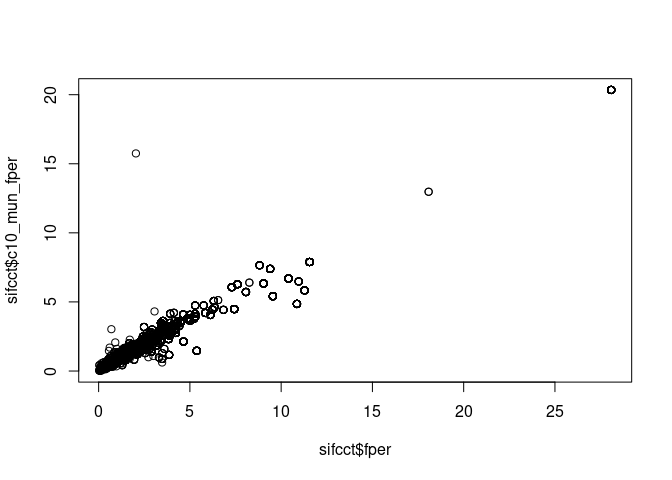
\includegraphics{visualization_1_descriptive_v5_files/figure-latex/unnamed-chunk-3-1.pdf}

\begin{Shaded}
\begin{Highlighting}[]
\KeywordTok{cor}\NormalTok{(sifcct}\OperatorTok{$}\NormalTok{fper, sifcct}\OperatorTok{$}\NormalTok{c10_mun_fper, }\DataTypeTok{use=}\StringTok{"pairwise"}\NormalTok{)}
\end{Highlighting}
\end{Shaded}

\begin{verbatim}
## [1] 0.972352
\end{verbatim}

\begin{Shaded}
\begin{Highlighting}[]
\KeywordTok{plot}\NormalTok{(sifcct}\OperatorTok{$}\NormalTok{c10_mun_fper, sifcct}\OperatorTok{$}\NormalTok{c10_sreg_fper)}
\end{Highlighting}
\end{Shaded}

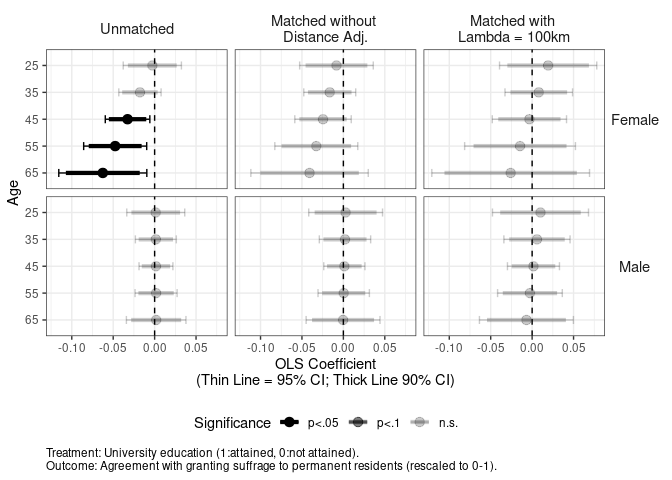
\includegraphics{visualization_1_descriptive_v5_files/figure-latex/unnamed-chunk-3-2.pdf}

\begin{Shaded}
\begin{Highlighting}[]
\KeywordTok{cor}\NormalTok{(sifcct}\OperatorTok{$}\NormalTok{c10_mun_fper, sifcct}\OperatorTok{$}\NormalTok{c10_sreg_fper, }\DataTypeTok{use=}\StringTok{"pairwise"}\NormalTok{)}
\end{Highlighting}
\end{Shaded}

\begin{verbatim}
## [1] 0.6087222
\end{verbatim}

\hypertarget{subset-data}{%
\section{Subset Data}\label{subset-data}}

\begin{Shaded}
\begin{Highlighting}[]
\NormalTok{sifcct_stayed <-}\StringTok{ }\KeywordTok{subset}\NormalTok{(sifcct, sifcct}\OperatorTok{$}\NormalTok{age }\OperatorTok{-}\StringTok{ }\NormalTok{sifcct}\OperatorTok{$}\NormalTok{lvlen}\OperatorTok{<=}\DecValTok{15}\NormalTok{)}
\NormalTok{sifcct_moved <-}\StringTok{ }\KeywordTok{subset}\NormalTok{(sifcct, sifcct}\OperatorTok{$}\NormalTok{age }\OperatorTok{-}\StringTok{ }\NormalTok{sifcct}\OperatorTok{$}\NormalTok{lvlen}\OperatorTok{>=}\DecValTok{23}\NormalTok{)}
\end{Highlighting}
\end{Shaded}

\hypertarget{education}{%
\section{Education}\label{education}}

\begin{Shaded}
\begin{Highlighting}[]
\NormalTok{tmp1 <-}\StringTok{ }\KeywordTok{t}\NormalTok{(}\KeywordTok{t}\NormalTok{(}\KeywordTok{table}\NormalTok{(sifcct_stayed[sifcct_stayed}\OperatorTok{$}\NormalTok{female}\OperatorTok{==}\DecValTok{1}\NormalTok{,]}\OperatorTok{$}\NormalTok{edu2, sifcct_stayed[sifcct_stayed}\OperatorTok{$}\NormalTok{female}\OperatorTok{==}\DecValTok{1}\NormalTok{,]}\OperatorTok{$}\NormalTok{agecat))}\OperatorTok{/}\KeywordTok{colSums}\NormalTok{(}\KeywordTok{table}\NormalTok{(sifcct_stayed[sifcct_stayed}\OperatorTok{$}\NormalTok{female}\OperatorTok{==}\DecValTok{1}\NormalTok{,]}\OperatorTok{$}\NormalTok{edu2, sifcct_stayed[sifcct_stayed}\OperatorTok{$}\NormalTok{female}\OperatorTok{==}\DecValTok{1}\NormalTok{,]}\OperatorTok{$}\NormalTok{agecat)))}
\NormalTok{tmp2 <-}\StringTok{ }\KeywordTok{t}\NormalTok{(}\KeywordTok{t}\NormalTok{(}\KeywordTok{table}\NormalTok{(sifcct_stayed[sifcct_stayed}\OperatorTok{$}\NormalTok{female}\OperatorTok{==}\DecValTok{0}\NormalTok{,]}\OperatorTok{$}\NormalTok{edu2, sifcct_stayed[sifcct_stayed}\OperatorTok{$}\NormalTok{female}\OperatorTok{==}\DecValTok{0}\NormalTok{,]}\OperatorTok{$}\NormalTok{agecat))}\OperatorTok{/}\KeywordTok{colSums}\NormalTok{(}\KeywordTok{table}\NormalTok{(sifcct_stayed[sifcct_stayed}\OperatorTok{$}\NormalTok{female}\OperatorTok{==}\DecValTok{0}\NormalTok{,]}\OperatorTok{$}\NormalTok{edu2, sifcct_stayed[sifcct_stayed}\OperatorTok{$}\NormalTok{female}\OperatorTok{==}\DecValTok{0}\NormalTok{,]}\OperatorTok{$}\NormalTok{agecat)))}
\NormalTok{tmp3 <-}\StringTok{ }\KeywordTok{t}\NormalTok{(}\KeywordTok{t}\NormalTok{(}\KeywordTok{table}\NormalTok{(sifcct_moved[sifcct_moved}\OperatorTok{$}\NormalTok{female}\OperatorTok{==}\DecValTok{1}\NormalTok{,]}\OperatorTok{$}\NormalTok{edu2, sifcct_moved[sifcct_moved}\OperatorTok{$}\NormalTok{female}\OperatorTok{==}\DecValTok{1}\NormalTok{,]}\OperatorTok{$}\NormalTok{agecat))}\OperatorTok{/}\KeywordTok{colSums}\NormalTok{(}\KeywordTok{table}\NormalTok{(sifcct_moved[sifcct_moved}\OperatorTok{$}\NormalTok{female}\OperatorTok{==}\DecValTok{1}\NormalTok{,]}\OperatorTok{$}\NormalTok{edu2, sifcct_moved[sifcct_moved}\OperatorTok{$}\NormalTok{female}\OperatorTok{==}\DecValTok{1}\NormalTok{,]}\OperatorTok{$}\NormalTok{agecat)))}
\NormalTok{tmp4 <-}\StringTok{ }\KeywordTok{t}\NormalTok{(}\KeywordTok{t}\NormalTok{(}\KeywordTok{table}\NormalTok{(sifcct_moved[sifcct_moved}\OperatorTok{$}\NormalTok{female}\OperatorTok{==}\DecValTok{0}\NormalTok{,]}\OperatorTok{$}\NormalTok{edu2, sifcct_moved[sifcct_moved}\OperatorTok{$}\NormalTok{female}\OperatorTok{==}\DecValTok{0}\NormalTok{,]}\OperatorTok{$}\NormalTok{agecat))}\OperatorTok{/}\KeywordTok{colSums}\NormalTok{(}\KeywordTok{table}\NormalTok{(sifcct_moved[sifcct_moved}\OperatorTok{$}\NormalTok{female}\OperatorTok{==}\DecValTok{0}\NormalTok{,]}\OperatorTok{$}\NormalTok{edu2, sifcct_moved[sifcct_moved}\OperatorTok{$}\NormalTok{female}\OperatorTok{==}\DecValTok{0}\NormalTok{,]}\OperatorTok{$}\NormalTok{agecat)))}

\NormalTok{pd <-}\StringTok{ }\KeywordTok{data.frame}\NormalTok{(}\DataTypeTok{prop=}\KeywordTok{c}\NormalTok{(tmp1[,}\DecValTok{1}\NormalTok{],tmp2[,}\DecValTok{1}\NormalTok{],tmp3[,}\DecValTok{1}\NormalTok{],tmp4[,}\DecValTok{1}\NormalTok{],}
\NormalTok{                        tmp1[,}\DecValTok{2}\NormalTok{],tmp2[,}\DecValTok{2}\NormalTok{],tmp3[,}\DecValTok{2}\NormalTok{],tmp4[,}\DecValTok{2}\NormalTok{],}
\NormalTok{                        tmp1[,}\DecValTok{3}\NormalTok{],tmp2[,}\DecValTok{3}\NormalTok{],tmp3[,}\DecValTok{3}\NormalTok{],tmp4[,}\DecValTok{3}\NormalTok{]))}
\NormalTok{pd}\OperatorTok{$}\NormalTok{gender <-}\StringTok{ }\KeywordTok{factor}\NormalTok{(}\KeywordTok{rep}\NormalTok{(}\KeywordTok{c}\NormalTok{(}\StringTok{"Female"}\NormalTok{,}\StringTok{"Male"}\NormalTok{),}\DataTypeTok{each=}\DecValTok{2}\NormalTok{), }\DataTypeTok{levels=}\KeywordTok{c}\NormalTok{(}\StringTok{"Female"}\NormalTok{,}\StringTok{"Male"}\NormalTok{))}
\NormalTok{pd}\OperatorTok{$}\NormalTok{cat <-}\StringTok{ }\KeywordTok{rep}\NormalTok{(}\KeywordTok{c}\NormalTok{(}\StringTok{"No"}\NormalTok{,}\StringTok{"Yes"}\NormalTok{),}\DataTypeTok{each=}\DecValTok{1}\NormalTok{)}
\NormalTok{pd}\OperatorTok{$}\NormalTok{cat <-}\StringTok{ }\KeywordTok{factor}\NormalTok{(pd}\OperatorTok{$}\NormalTok{cat, }\DataTypeTok{levels=}\KeywordTok{unique}\NormalTok{(pd}\OperatorTok{$}\NormalTok{cat))}
\NormalTok{pd}\OperatorTok{$}\NormalTok{sample <-}\StringTok{ }\KeywordTok{rep}\NormalTok{(}\KeywordTok{c}\NormalTok{(}\StringTok{"Stayed"}\NormalTok{,}\StringTok{"Moved"}\NormalTok{),}\DataTypeTok{each=}\DecValTok{4}\NormalTok{)}
\NormalTok{pd}\OperatorTok{$}\NormalTok{sample <-}\StringTok{ }\KeywordTok{factor}\NormalTok{(pd}\OperatorTok{$}\NormalTok{sample, }\DataTypeTok{levels=}\KeywordTok{unique}\NormalTok{(pd}\OperatorTok{$}\NormalTok{sample))}
\NormalTok{pd}\OperatorTok{$}\NormalTok{agecat <-}\StringTok{ }\KeywordTok{rep}\NormalTok{(}\KeywordTok{c}\NormalTok{(}\StringTok{"Young}\CharTok{\textbackslash{}n}\StringTok{(<=30s)"}\NormalTok{,}
                   \StringTok{"Middle Aged}\CharTok{\textbackslash{}n}\StringTok{(40-50s)"}\NormalTok{,}\StringTok{"Elder}\CharTok{\textbackslash{}n}\StringTok{(>=60s)"}\NormalTok{),}\DataTypeTok{each=}\DecValTok{8}\NormalTok{)}
\NormalTok{pd}\OperatorTok{$}\NormalTok{agecat <-}\StringTok{ }\KeywordTok{factor}\NormalTok{(pd}\OperatorTok{$}\NormalTok{agecat, }\DataTypeTok{levels=}\KeywordTok{unique}\NormalTok{(pd}\OperatorTok{$}\NormalTok{agecat))}

\CommentTok{# Plot}
\NormalTok{p <-}\StringTok{ }\KeywordTok{ggplot}\NormalTok{(}\DataTypeTok{data=}\NormalTok{pd, }\KeywordTok{aes}\NormalTok{(}\DataTypeTok{x=}\NormalTok{cat,}\DataTypeTok{y=}\NormalTok{prop)) }\OperatorTok{+}\StringTok{ }
\StringTok{  }\KeywordTok{geom_col}\NormalTok{(}\KeywordTok{aes}\NormalTok{(}\DataTypeTok{fill=}\NormalTok{sample), }\DataTypeTok{color =} \StringTok{"gray50"}\NormalTok{, }\DataTypeTok{position=}\KeywordTok{position_dodge}\NormalTok{(}\DataTypeTok{width=}\OperatorTok{-}\FloatTok{0.9}\NormalTok{)) }\OperatorTok{+}\StringTok{  }
\StringTok{  }\KeywordTok{facet_grid}\NormalTok{(gender}\OperatorTok{~}\NormalTok{agecat, }\DataTypeTok{scale=}\StringTok{"free_x"}\NormalTok{) }\OperatorTok{+}
\StringTok{  }\CommentTok{#coord_flip() + }
\StringTok{  }\KeywordTok{xlab}\NormalTok{(}\StringTok{"University Degree"}\NormalTok{) }\OperatorTok{+}\StringTok{ }\KeywordTok{ylab}\NormalTok{(}\StringTok{"Proportion within Gender"}\NormalTok{) }\OperatorTok{+}
\StringTok{  }\KeywordTok{scale_fill_brewer}\NormalTok{(}\DataTypeTok{name=}\StringTok{"Residence Before & After Age 15-23"}\NormalTok{, }\DataTypeTok{type =} \StringTok{"seq"}\NormalTok{, }\DataTypeTok{palette =} \DecValTok{3}\NormalTok{) }\OperatorTok{+}\StringTok{ }
\StringTok{  }\KeywordTok{scale_y_continuous}\NormalTok{(}\DataTypeTok{limits=}\KeywordTok{c}\NormalTok{(}\DecValTok{0}\NormalTok{,}\FloatTok{0.85}\NormalTok{)) }\OperatorTok{+}
\StringTok{  }\KeywordTok{theme_bw}\NormalTok{() }\OperatorTok{+}\StringTok{ }
\StringTok{  }\KeywordTok{theme}\NormalTok{(}\DataTypeTok{legend.position =} \StringTok{"bottom"}\NormalTok{,}
        \DataTypeTok{strip.text.x =} \KeywordTok{element_text}\NormalTok{(}\DataTypeTok{size=}\DecValTok{11}\NormalTok{),}
        \DataTypeTok{strip.text.y =} \KeywordTok{element_text}\NormalTok{(}\DataTypeTok{angle=}\DecValTok{0}\NormalTok{,}\DataTypeTok{size=}\DecValTok{11}\NormalTok{),}
        \DataTypeTok{strip.background =} \KeywordTok{element_rect}\NormalTok{(}\DataTypeTok{fill=}\OtherTok{NA}\NormalTok{,}\DataTypeTok{color=}\OtherTok{NA}\NormalTok{),}
        \DataTypeTok{plot.caption =} \KeywordTok{element_text}\NormalTok{(}\DataTypeTok{hjust=}\DecValTok{0}\NormalTok{),}
        \DataTypeTok{plot.caption.position =} \StringTok{"plot"}\NormalTok{,}
        \DataTypeTok{axis.text.y =} \KeywordTok{element_text}\NormalTok{(}\DataTypeTok{size=}\DecValTok{10}\NormalTok{, }\DataTypeTok{color=}\StringTok{"black"}\NormalTok{))}
\end{Highlighting}
\end{Shaded}

\begin{Shaded}
\begin{Highlighting}[]
\NormalTok{p}
\end{Highlighting}
\end{Shaded}

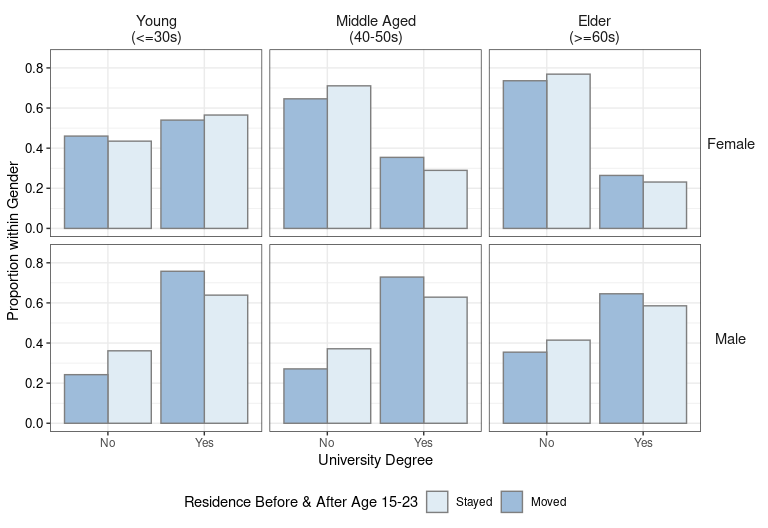
\includegraphics{visualization_1_descriptive_v5_files/figure-latex/unnamed-chunk-6-1.pdf}

\begin{Shaded}
\begin{Highlighting}[]
\KeywordTok{ggsave}\NormalTok{(}\KeywordTok{paste0}\NormalTok{(projdir,}\StringTok{"/out/descrplot_edu2.png"}\NormalTok{),p, }\DataTypeTok{width=}\DecValTok{8}\NormalTok{, }\DataTypeTok{height=}\FloatTok{5.5}\NormalTok{)}
\KeywordTok{ggsave}\NormalTok{(}\KeywordTok{paste0}\NormalTok{(projdir,}\StringTok{"/out/descrplot_edu2.pdf"}\NormalTok{),p, }\DataTypeTok{width=}\DecValTok{8}\NormalTok{, }\DataTypeTok{height=}\FloatTok{5.5}\NormalTok{)}
\end{Highlighting}
\end{Shaded}

\hypertarget{outcome-policy-variable}{%
\section{Outcome Policy Variable}\label{outcome-policy-variable}}

\begin{Shaded}
\begin{Highlighting}[]
\CommentTok{# Plotting Data}
\NormalTok{tmp1 <-}\StringTok{ }\KeywordTok{t}\NormalTok{(}\KeywordTok{t}\NormalTok{(}\KeywordTok{table}\NormalTok{(sifcct_stayed[sifcct_stayed}\OperatorTok{$}\NormalTok{female}\OperatorTok{==}\DecValTok{1}\NormalTok{,]}\OperatorTok{$}\NormalTok{foreignsuff, sifcct_stayed[sifcct_stayed}\OperatorTok{$}\NormalTok{female}\OperatorTok{==}\DecValTok{1}\NormalTok{,]}\OperatorTok{$}\NormalTok{agecat))}\OperatorTok{/}\KeywordTok{colSums}\NormalTok{(}\KeywordTok{table}\NormalTok{(sifcct_stayed[sifcct_stayed}\OperatorTok{$}\NormalTok{female}\OperatorTok{==}\DecValTok{1}\NormalTok{,]}\OperatorTok{$}\NormalTok{foreignsuff, sifcct_stayed[sifcct_stayed}\OperatorTok{$}\NormalTok{female}\OperatorTok{==}\DecValTok{1}\NormalTok{,]}\OperatorTok{$}\NormalTok{agecat)))}
\NormalTok{tmp2 <-}\StringTok{ }\KeywordTok{t}\NormalTok{(}\KeywordTok{t}\NormalTok{(}\KeywordTok{table}\NormalTok{(sifcct_stayed[sifcct_stayed}\OperatorTok{$}\NormalTok{female}\OperatorTok{==}\DecValTok{0}\NormalTok{,]}\OperatorTok{$}\NormalTok{foreignsuff, sifcct_stayed[sifcct_stayed}\OperatorTok{$}\NormalTok{female}\OperatorTok{==}\DecValTok{0}\NormalTok{,]}\OperatorTok{$}\NormalTok{agecat))}\OperatorTok{/}\KeywordTok{colSums}\NormalTok{(}\KeywordTok{table}\NormalTok{(sifcct_stayed[sifcct_stayed}\OperatorTok{$}\NormalTok{female}\OperatorTok{==}\DecValTok{0}\NormalTok{,]}\OperatorTok{$}\NormalTok{foreignsuff, sifcct_stayed[sifcct_stayed}\OperatorTok{$}\NormalTok{female}\OperatorTok{==}\DecValTok{0}\NormalTok{,]}\OperatorTok{$}\NormalTok{agecat)))}
\NormalTok{tmp3 <-}\StringTok{ }\KeywordTok{t}\NormalTok{(}\KeywordTok{t}\NormalTok{(}\KeywordTok{table}\NormalTok{(sifcct_moved[sifcct_moved}\OperatorTok{$}\NormalTok{female}\OperatorTok{==}\DecValTok{1}\NormalTok{,]}\OperatorTok{$}\NormalTok{foreignsuff, sifcct_moved[sifcct_moved}\OperatorTok{$}\NormalTok{female}\OperatorTok{==}\DecValTok{1}\NormalTok{,]}\OperatorTok{$}\NormalTok{agecat))}\OperatorTok{/}\KeywordTok{colSums}\NormalTok{(}\KeywordTok{table}\NormalTok{(sifcct_moved[sifcct_moved}\OperatorTok{$}\NormalTok{female}\OperatorTok{==}\DecValTok{1}\NormalTok{,]}\OperatorTok{$}\NormalTok{foreignsuff, sifcct_moved[sifcct_moved}\OperatorTok{$}\NormalTok{female}\OperatorTok{==}\DecValTok{1}\NormalTok{,]}\OperatorTok{$}\NormalTok{agecat)))}
\NormalTok{tmp4 <-}\StringTok{ }\KeywordTok{t}\NormalTok{(}\KeywordTok{t}\NormalTok{(}\KeywordTok{table}\NormalTok{(sifcct_moved[sifcct_moved}\OperatorTok{$}\NormalTok{female}\OperatorTok{==}\DecValTok{0}\NormalTok{,]}\OperatorTok{$}\NormalTok{foreignsuff, sifcct_moved[sifcct_moved}\OperatorTok{$}\NormalTok{female}\OperatorTok{==}\DecValTok{0}\NormalTok{,]}\OperatorTok{$}\NormalTok{agecat))}\OperatorTok{/}\KeywordTok{colSums}\NormalTok{(}\KeywordTok{table}\NormalTok{(sifcct_moved[sifcct_moved}\OperatorTok{$}\NormalTok{female}\OperatorTok{==}\DecValTok{0}\NormalTok{,]}\OperatorTok{$}\NormalTok{foreignsuff, sifcct_moved[sifcct_moved}\OperatorTok{$}\NormalTok{female}\OperatorTok{==}\DecValTok{0}\NormalTok{,]}\OperatorTok{$}\NormalTok{agecat)))}

\NormalTok{pd <-}\StringTok{ }\KeywordTok{data.frame}\NormalTok{(}\DataTypeTok{prop=}\KeywordTok{c}\NormalTok{(tmp1[,}\DecValTok{1}\NormalTok{],tmp2[,}\DecValTok{1}\NormalTok{],tmp3[,}\DecValTok{1}\NormalTok{],tmp4[,}\DecValTok{1}\NormalTok{],}
\NormalTok{                        tmp1[,}\DecValTok{2}\NormalTok{],tmp2[,}\DecValTok{2}\NormalTok{],tmp3[,}\DecValTok{2}\NormalTok{],tmp4[,}\DecValTok{2}\NormalTok{],}
\NormalTok{                        tmp1[,}\DecValTok{3}\NormalTok{],tmp2[,}\DecValTok{3}\NormalTok{],tmp3[,}\DecValTok{3}\NormalTok{],tmp4[,}\DecValTok{3}\NormalTok{]))}
\NormalTok{pd}\OperatorTok{$}\NormalTok{gender <-}\StringTok{ }\KeywordTok{factor}\NormalTok{(}\KeywordTok{rep}\NormalTok{(}\KeywordTok{c}\NormalTok{(}\StringTok{"Female"}\NormalTok{,}\StringTok{"Male"}\NormalTok{),}\DataTypeTok{each=}\DecValTok{5}\NormalTok{), }\DataTypeTok{levels=}\KeywordTok{c}\NormalTok{(}\StringTok{"Female"}\NormalTok{,}\StringTok{"Male"}\NormalTok{))}
\NormalTok{pd}\OperatorTok{$}\NormalTok{cat <-}\StringTok{ }\KeywordTok{c}\NormalTok{(}\StringTok{"Strongly Disagree"}\NormalTok{,}\StringTok{"Disagree"}\NormalTok{,}\StringTok{"Neither/DK"}\NormalTok{,}\StringTok{"Agree"}\NormalTok{,}\StringTok{"Strongly Agree"}\NormalTok{)}
\NormalTok{pd}\OperatorTok{$}\NormalTok{cat <-}\StringTok{ }\KeywordTok{factor}\NormalTok{(pd}\OperatorTok{$}\NormalTok{cat, }\DataTypeTok{levels=}\NormalTok{(}\KeywordTok{unique}\NormalTok{(pd}\OperatorTok{$}\NormalTok{cat)))}
\NormalTok{pd}\OperatorTok{$}\NormalTok{num <-}\StringTok{ }\KeywordTok{as.numeric}\NormalTok{(}\KeywordTok{names}\NormalTok{(}\KeywordTok{table}\NormalTok{(sifcct}\OperatorTok{$}\NormalTok{foreignsuff)))}
\NormalTok{pd}\OperatorTok{$}\NormalTok{num <-}\StringTok{ }\KeywordTok{factor}\NormalTok{(pd}\OperatorTok{$}\NormalTok{num, }\DataTypeTok{levels=}\NormalTok{(}\KeywordTok{unique}\NormalTok{(pd}\OperatorTok{$}\NormalTok{num)))}
\NormalTok{pd}\OperatorTok{$}\NormalTok{sample <-}\StringTok{ }\KeywordTok{rep}\NormalTok{(}\KeywordTok{c}\NormalTok{(}\StringTok{"Stayed"}\NormalTok{,}\StringTok{"Moved"}\NormalTok{),}\DataTypeTok{each=}\DecValTok{10}\NormalTok{)}
\NormalTok{pd}\OperatorTok{$}\NormalTok{sample <-}\StringTok{ }\KeywordTok{factor}\NormalTok{(pd}\OperatorTok{$}\NormalTok{sample, }\DataTypeTok{levels=}\KeywordTok{unique}\NormalTok{(pd}\OperatorTok{$}\NormalTok{sample))}
\NormalTok{pd}\OperatorTok{$}\NormalTok{agecat <-}\StringTok{ }\KeywordTok{rep}\NormalTok{(}\KeywordTok{c}\NormalTok{(}\StringTok{"Young}\CharTok{\textbackslash{}n}\StringTok{(<=30s)"}\NormalTok{,}\StringTok{"Middle Aged}\CharTok{\textbackslash{}n}\StringTok{(40-50s)"}\NormalTok{,}\StringTok{"Elder}\CharTok{\textbackslash{}n}\StringTok{(>=60s)"}\NormalTok{),}\DataTypeTok{each=}\DecValTok{20}\NormalTok{)}
\NormalTok{pd}\OperatorTok{$}\NormalTok{agecat <-}\StringTok{ }\KeywordTok{factor}\NormalTok{(pd}\OperatorTok{$}\NormalTok{agecat, }\DataTypeTok{levels=}\KeywordTok{unique}\NormalTok{(pd}\OperatorTok{$}\NormalTok{agecat))}

\CommentTok{# Plot}
\NormalTok{p <-}\StringTok{ }\KeywordTok{ggplot}\NormalTok{(}\DataTypeTok{data=}\NormalTok{pd, }\KeywordTok{aes}\NormalTok{(}\DataTypeTok{x=}\NormalTok{num,}\DataTypeTok{y=}\NormalTok{prop)) }\OperatorTok{+}\StringTok{ }
\StringTok{  }\KeywordTok{geom_col}\NormalTok{(}\KeywordTok{aes}\NormalTok{(}\DataTypeTok{fill=}\NormalTok{sample), }\DataTypeTok{color =} \StringTok{"gray50"}\NormalTok{, }\DataTypeTok{position=}\KeywordTok{position_dodge}\NormalTok{(}\DataTypeTok{width=}\OperatorTok{-}\FloatTok{0.9}\NormalTok{)) }\OperatorTok{+}\StringTok{  }
\StringTok{  }\KeywordTok{facet_grid}\NormalTok{(gender}\OperatorTok{~}\NormalTok{agecat, }\DataTypeTok{scale=}\StringTok{"free_x"}\NormalTok{) }\OperatorTok{+}
\StringTok{  }\CommentTok{# coord_flip() + }
\StringTok{  }\KeywordTok{xlab}\NormalTok{(}\StringTok{"Granting Suffrage to Permanent Residents}\CharTok{\textbackslash{}n}\StringTok{(0 = Strongly Disagree, 1 = Strongly Agree)"}\NormalTok{) }\OperatorTok{+}\StringTok{ }
\StringTok{  }\KeywordTok{ylab}\NormalTok{(}\StringTok{"Proportion within Gender"}\NormalTok{) }\OperatorTok{+}
\StringTok{  }\KeywordTok{scale_fill_brewer}\NormalTok{(}\DataTypeTok{name=}\StringTok{"Residence Before & After Age 15-23"}\NormalTok{, }\DataTypeTok{type =} \StringTok{"seq"}\NormalTok{, }\DataTypeTok{palette =} \DecValTok{3}\NormalTok{) }\OperatorTok{+}\StringTok{ }
\StringTok{  }\CommentTok{# scale_y_continuous(limits=c(0,0.7)) +}
\StringTok{  }\KeywordTok{scale_x_discrete}\NormalTok{(}\DataTypeTok{labels=}\KeywordTok{c}\NormalTok{(}\StringTok{"0"}\NormalTok{,}\StringTok{""}\NormalTok{,}\StringTok{"0.5"}\NormalTok{,}\StringTok{""}\NormalTok{,}\StringTok{"1"}\NormalTok{)) }\OperatorTok{+}\StringTok{ }
\StringTok{  }\KeywordTok{theme_bw}\NormalTok{() }\OperatorTok{+}\StringTok{ }
\StringTok{  }\KeywordTok{theme}\NormalTok{(}\DataTypeTok{legend.position =} \StringTok{"bottom"}\NormalTok{,}
        \DataTypeTok{strip.text.x =} \KeywordTok{element_text}\NormalTok{(}\DataTypeTok{size=}\DecValTok{11}\NormalTok{),}
        \DataTypeTok{strip.text.y =} \KeywordTok{element_text}\NormalTok{(}\DataTypeTok{angle=}\DecValTok{0}\NormalTok{,}\DataTypeTok{size=}\DecValTok{11}\NormalTok{),}
        \DataTypeTok{strip.background =} \KeywordTok{element_rect}\NormalTok{(}\DataTypeTok{fill=}\OtherTok{NA}\NormalTok{,}\DataTypeTok{color=}\OtherTok{NA}\NormalTok{),}
        \DataTypeTok{plot.caption =} \KeywordTok{element_text}\NormalTok{(}\DataTypeTok{hjust=}\DecValTok{0}\NormalTok{),}
        \DataTypeTok{plot.caption.position =} \StringTok{"plot"}\NormalTok{,}
        \DataTypeTok{axis.text.y =} \KeywordTok{element_text}\NormalTok{(}\DataTypeTok{size=}\DecValTok{10}\NormalTok{, }\DataTypeTok{color=}\StringTok{"black"}\NormalTok{))}
\end{Highlighting}
\end{Shaded}

\begin{Shaded}
\begin{Highlighting}[]
\NormalTok{p}
\end{Highlighting}
\end{Shaded}

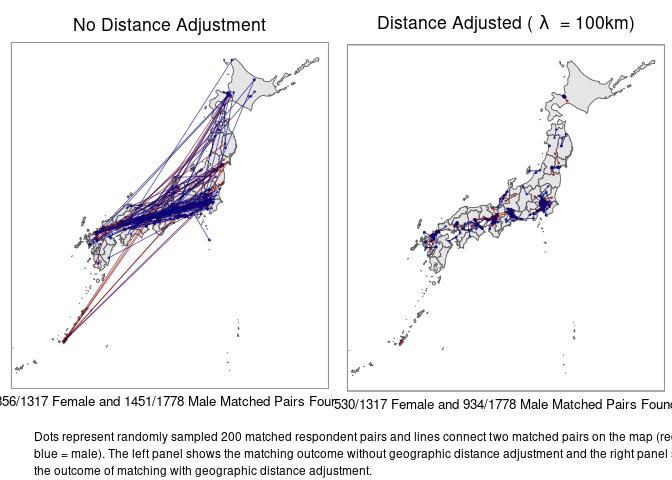
\includegraphics{visualization_1_descriptive_v5_files/figure-latex/unnamed-chunk-9-1.pdf}

\begin{Shaded}
\begin{Highlighting}[]
\KeywordTok{ggsave}\NormalTok{(}\KeywordTok{paste0}\NormalTok{(projdir,}\StringTok{"/out/descrplot_out.png"}\NormalTok{),p, }\DataTypeTok{width=}\DecValTok{8}\NormalTok{, }\DataTypeTok{height=}\FloatTok{5.5}\NormalTok{)}
\KeywordTok{ggsave}\NormalTok{(}\KeywordTok{paste0}\NormalTok{(projdir,}\StringTok{"/out/descrplot_out.pdf"}\NormalTok{),p, }\DataTypeTok{width=}\DecValTok{8}\NormalTok{, }\DataTypeTok{height=}\FloatTok{5.5}\NormalTok{)}
\end{Highlighting}
\end{Shaded}

\hypertarget{mediator-variables}{%
\section{Mediator Variables}\label{mediator-variables}}

\begin{Shaded}
\begin{Highlighting}[]
\CommentTok{# Data}
\NormalTok{pd <-}\StringTok{ }\KeywordTok{data.frame}\NormalTok{(}\DataTypeTok{med =} \KeywordTok{c}\NormalTok{(sifcct_stayed}\OperatorTok{$}\NormalTok{income,sifcct_moved}\OperatorTok{$}\NormalTok{income,}
\NormalTok{                         sifcct_stayed}\OperatorTok{$}\NormalTok{ideology,sifcct_moved}\OperatorTok{$}\NormalTok{ideology,}
\NormalTok{                         sifcct_stayed}\OperatorTok{$}\NormalTok{ldpdpjft,sifcct_moved}\OperatorTok{$}\NormalTok{ldpdpjft,}
\NormalTok{                         sifcct_stayed}\OperatorTok{$}\NormalTok{familiarityFT_KOR,sifcct_moved}\OperatorTok{$}\NormalTok{familiarityFT_KOR,}
\NormalTok{                         sifcct_stayed}\OperatorTok{$}\NormalTok{familiarityFT_CHN,sifcct_moved}\OperatorTok{$}\NormalTok{familiarityFT_CHN,}
\NormalTok{                         sifcct_stayed}\OperatorTok{$}\NormalTok{familiarityFT_USA,sifcct_moved}\OperatorTok{$}\NormalTok{familiarityFT_USA),}
                 \DataTypeTok{sample =} \KeywordTok{c}\NormalTok{(}\KeywordTok{rep}\NormalTok{(}\StringTok{"Stayed"}\NormalTok{,}\KeywordTok{nrow}\NormalTok{(sifcct_stayed)),}
                            \KeywordTok{rep}\NormalTok{(}\StringTok{"Moved"}\NormalTok{,}\KeywordTok{nrow}\NormalTok{(sifcct_moved))),}
                 \DataTypeTok{vn =} \KeywordTok{rep}\NormalTok{(}\KeywordTok{c}\NormalTok{(}\StringTok{"Income"}\NormalTok{,}\StringTok{"Ideology"}\NormalTok{,}\StringTok{"LDP-DPJ FT"}\NormalTok{, }
                            \StringTok{"Korea FT"}\NormalTok{, }\StringTok{"China FT"}\NormalTok{, }\StringTok{"US FT"}\NormalTok{),}
                          \DataTypeTok{each =} \KeywordTok{nrow}\NormalTok{(sifcct_stayed) }\OperatorTok{+}\StringTok{ }\KeywordTok{nrow}\NormalTok{(sifcct_moved)))}
\NormalTok{pd}\OperatorTok{$}\NormalTok{vn <-}\StringTok{ }\KeywordTok{factor}\NormalTok{(pd}\OperatorTok{$}\NormalTok{vn, }\DataTypeTok{levels=}\KeywordTok{unique}\NormalTok{(pd}\OperatorTok{$}\NormalTok{vn))}

\CommentTok{# Plot}
\KeywordTok{require}\NormalTok{(ggplot2)}
\NormalTok{p <-}\StringTok{ }\KeywordTok{ggplot}\NormalTok{(}\DataTypeTok{data =}\NormalTok{ pd, }\KeywordTok{aes}\NormalTok{(}\DataTypeTok{x=}\NormalTok{med,}\DataTypeTok{y=}\NormalTok{..density..)) }\OperatorTok{+}\StringTok{ }
\StringTok{  }\KeywordTok{geom_histogram}\NormalTok{(}\KeywordTok{aes}\NormalTok{(}\DataTypeTok{fill=}\NormalTok{sample), }\DataTypeTok{color =} \StringTok{"gray50"}\NormalTok{, }
                 \DataTypeTok{position=}\KeywordTok{position_dodge}\NormalTok{(}\DataTypeTok{width=}\FloatTok{0.15}\NormalTok{),}
                 \DataTypeTok{binwidth =} \FloatTok{0.2}\NormalTok{) }\OperatorTok{+}
\StringTok{  }\KeywordTok{facet_wrap}\NormalTok{(pd}\OperatorTok{$}\NormalTok{vn) }\OperatorTok{+}\StringTok{ }
\StringTok{  }\KeywordTok{xlab}\NormalTok{(}\StringTok{"Normalized Values (Histogram) }\CharTok{\textbackslash{}n}\StringTok{0: Low/Liberal/Cold to 1: High/Conservative/Warm"}\NormalTok{) }\OperatorTok{+}
\StringTok{  }\KeywordTok{ylab}\NormalTok{(}\StringTok{"Density"}\NormalTok{) }\OperatorTok{+}
\StringTok{  }\KeywordTok{scale_fill_brewer}\NormalTok{(}\DataTypeTok{name=}\StringTok{"Residence Before & After Age 15-23"}\NormalTok{, }\DataTypeTok{type =} \StringTok{"seq"}\NormalTok{, }\DataTypeTok{palette =} \DecValTok{3}\NormalTok{) }\OperatorTok{+}
\StringTok{  }\KeywordTok{scale_x_continuous}\NormalTok{(}\DataTypeTok{limits=}\KeywordTok{c}\NormalTok{(}\OperatorTok{-}\FloatTok{0.1}\NormalTok{,}\FloatTok{1.1}\NormalTok{), }\DataTypeTok{breaks=}\KeywordTok{seq}\NormalTok{(}\DecValTok{0}\NormalTok{,}\DecValTok{1}\NormalTok{,}\DataTypeTok{by=}\FloatTok{0.2}\NormalTok{)) }\OperatorTok{+}
\StringTok{  }\CommentTok{# scale_x_discrete(labels=c("0","","0.5","","1")) +}
\StringTok{  }\KeywordTok{theme_bw}\NormalTok{() }\OperatorTok{+}
\StringTok{  }\KeywordTok{theme}\NormalTok{(}\DataTypeTok{legend.position =} \StringTok{"bottom"}\NormalTok{,}
        \DataTypeTok{strip.text.x =} \KeywordTok{element_text}\NormalTok{(}\DataTypeTok{size=}\DecValTok{11}\NormalTok{),}
        \DataTypeTok{strip.text.y =} \KeywordTok{element_text}\NormalTok{(}\DataTypeTok{angle=}\DecValTok{0}\NormalTok{,}\DataTypeTok{size=}\DecValTok{11}\NormalTok{),}
        \DataTypeTok{strip.background =} \KeywordTok{element_rect}\NormalTok{(}\DataTypeTok{fill=}\OtherTok{NA}\NormalTok{,}\DataTypeTok{color=}\OtherTok{NA}\NormalTok{),}
        \DataTypeTok{plot.caption =} \KeywordTok{element_text}\NormalTok{(}\DataTypeTok{hjust=}\DecValTok{0}\NormalTok{),}
        \DataTypeTok{plot.caption.position =} \StringTok{"plot"}\NormalTok{,}
        \DataTypeTok{axis.text.y =} \KeywordTok{element_text}\NormalTok{(}\DataTypeTok{size=}\DecValTok{10}\NormalTok{, }\DataTypeTok{color=}\StringTok{"black"}\NormalTok{))}
\end{Highlighting}
\end{Shaded}

\begin{Shaded}
\begin{Highlighting}[]
\NormalTok{p}
\end{Highlighting}
\end{Shaded}

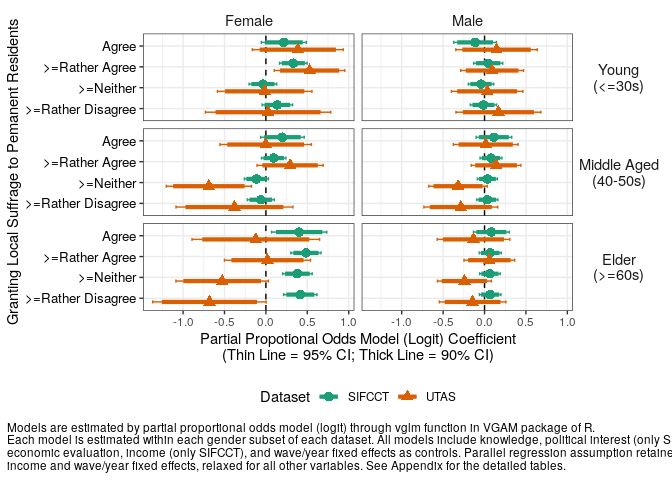
\includegraphics{visualization_1_descriptive_v5_files/figure-latex/unnamed-chunk-12-1.pdf}

\begin{Shaded}
\begin{Highlighting}[]
\KeywordTok{ggsave}\NormalTok{(}\KeywordTok{paste0}\NormalTok{(projdir,}\StringTok{"/out/descrplot_med.png"}\NormalTok{),p, }\DataTypeTok{width=}\DecValTok{8}\NormalTok{, }\DataTypeTok{height=}\FloatTok{5.5}\NormalTok{)}
\KeywordTok{ggsave}\NormalTok{(}\KeywordTok{paste0}\NormalTok{(projdir,}\StringTok{"/out/descrplot_med.pdf"}\NormalTok{),p, }\DataTypeTok{width=}\DecValTok{8}\NormalTok{, }\DataTypeTok{height=}\FloatTok{5.5}\NormalTok{)}
\end{Highlighting}
\end{Shaded}

\end{document}
